% TemplateV5.tex --  LaTeX-based template for submissions to the American Meteorological Society
% Version 5.0, 2 January 2020

% Paper layout
%\documentclass{ametsocV5} %for submission
\documentclass[twocol]{ametsocV5} % two-column layout (for author use only)

% Packages
\usepackage{amsmath,amsfonts,amssymb,bm}
\usepackage{mathptmx}
\usepackage{newtxtext}
\usepackage{newtxmath}
\usepackage{enumitem}
\usepackage{multirow}
\usepackage{amsmath}



%%%%%%%%%
% TITLE %
%%%%%%%%%
\title{Operational adoption of new probabilistic point rainfall forecasts: the crucial role of a user-centric training}


%%%%%%%%%%%
% AUTHORS %
%%%%%%%%%%%

\authors{Fatima M. Pillosu\correspondingauthor{Fatima Pillosu, fatima.pillosu@ecmwf.int}}
\affiliation{University of Reading, Reading, UK \\
European Centre for Medium-Range Weather Forecasts, Reading, UK}

\extraauthor{Boglárka Tóth, Istvan Ihasz}
\extraaffil{Hungarian Meteorological Service, Budapest, Hungary}

\extraauthor{Roberto Vindas Morán, Werner Stolz}
\extraaffil{National Meteorological Institute of Costa Rica, San José, Costa Rica}

\extraauthor{Tim Hewson}
\extraaffil{European Centre for Medium-Range Weather Forecasts, Reading, UK}

\extraauthor{Christel Prudhomme}
\extraaffil{European Centre for Medium-Range Weather Forecasts, Reading, UK \\
Loughborough University, Loughborough, UK}

\extraauthor{Elisabeth Stephens}
\extraaffil{University of Reading, Reading, UK}

\extraauthor{Hannah L. Cloke}
\extraaffil{University of Reading, Reading, UK \\
Uppsala University, Uppsala, Sweden \\
Centre of Natural hazards and Disaster Science, Uppsala, Sweden}



%%%%%%%%%%%%
% ABSTRACT %
%%%%%%%%%%%%
\abstract{}


%%%%%%%%%%%%%%%%%%%%%%
% MAIN BODY OF PAPER %
%%%%%%%%%%%%%%%%%%%%%%
\begin{document}
\maketitle


%%%%%%%%%%%%%%%%%%%%
% INTRODUCTION
\section{Introduction}




%%%%%%%%%%%%%%%%%%%%
% ecPoint-Rainfall

\section{ecPoint-Rainfall}

\begin{sidewaysfigure*}
\centerline{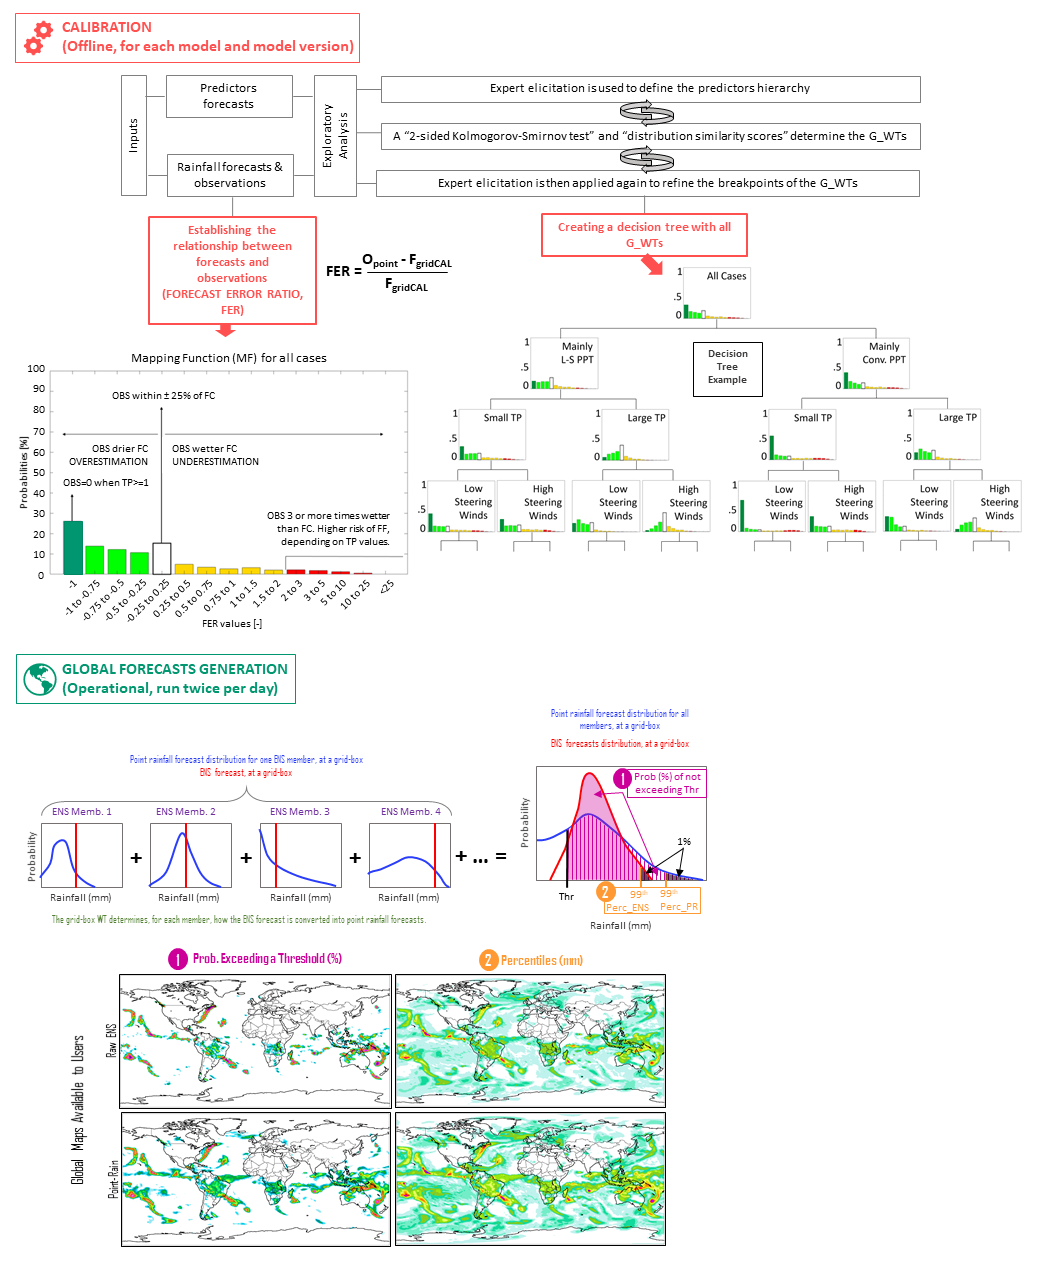
\includegraphics[width=53pc]{manuscript/Figures/ecPoint_Methodology.png}}
\caption{ecPoint Workflow. The left (red) panel represents the ecPoint's offline calibration process. The right (green) panel represents the ecPoint's forecast generation process and the products that can be derived from the post-processing output. The variable "rainfall" was used in this figure two illustrate both processes, calibration and forecast generation, but they can be used to post-process also other variables, e.g. "temperature".}
\label{ecPoint_Methodology}
\end{sidewaysfigure*}




%%%%%%%%%%%%%%%%%%%%
% Background of ecPoint-Rainfall testers

\begin{figure}
\centerline{\includegraphics[width=19pc]{manuscript/Figures/GeoLocation_H_CR.png}}
\caption{Panel (a) shows Costa Rica location in Central America and Hungary location in Europe. Panel (b) and (c) show respectively the orography of Costa Rica and Hungary.}
\label{GeoLocation_H_CR}
\end{figure}

\section{Background on Costa Rica}
\subsection{Extreme rainfall climatology in Costa Rica}
\subsection{How does IMN traditionally forecast extreme rainfall events?}

\section{Background on Hungary}
\subsection{Extreme rainfall climatology in Hungary}
\subsection{How does OMSZ traditionally forecast extreme rainfall events?}




%%%%%%%%%%%%%%%%%%%%
% Methods
\section{Methods} 

\begin{figure}
\centerline{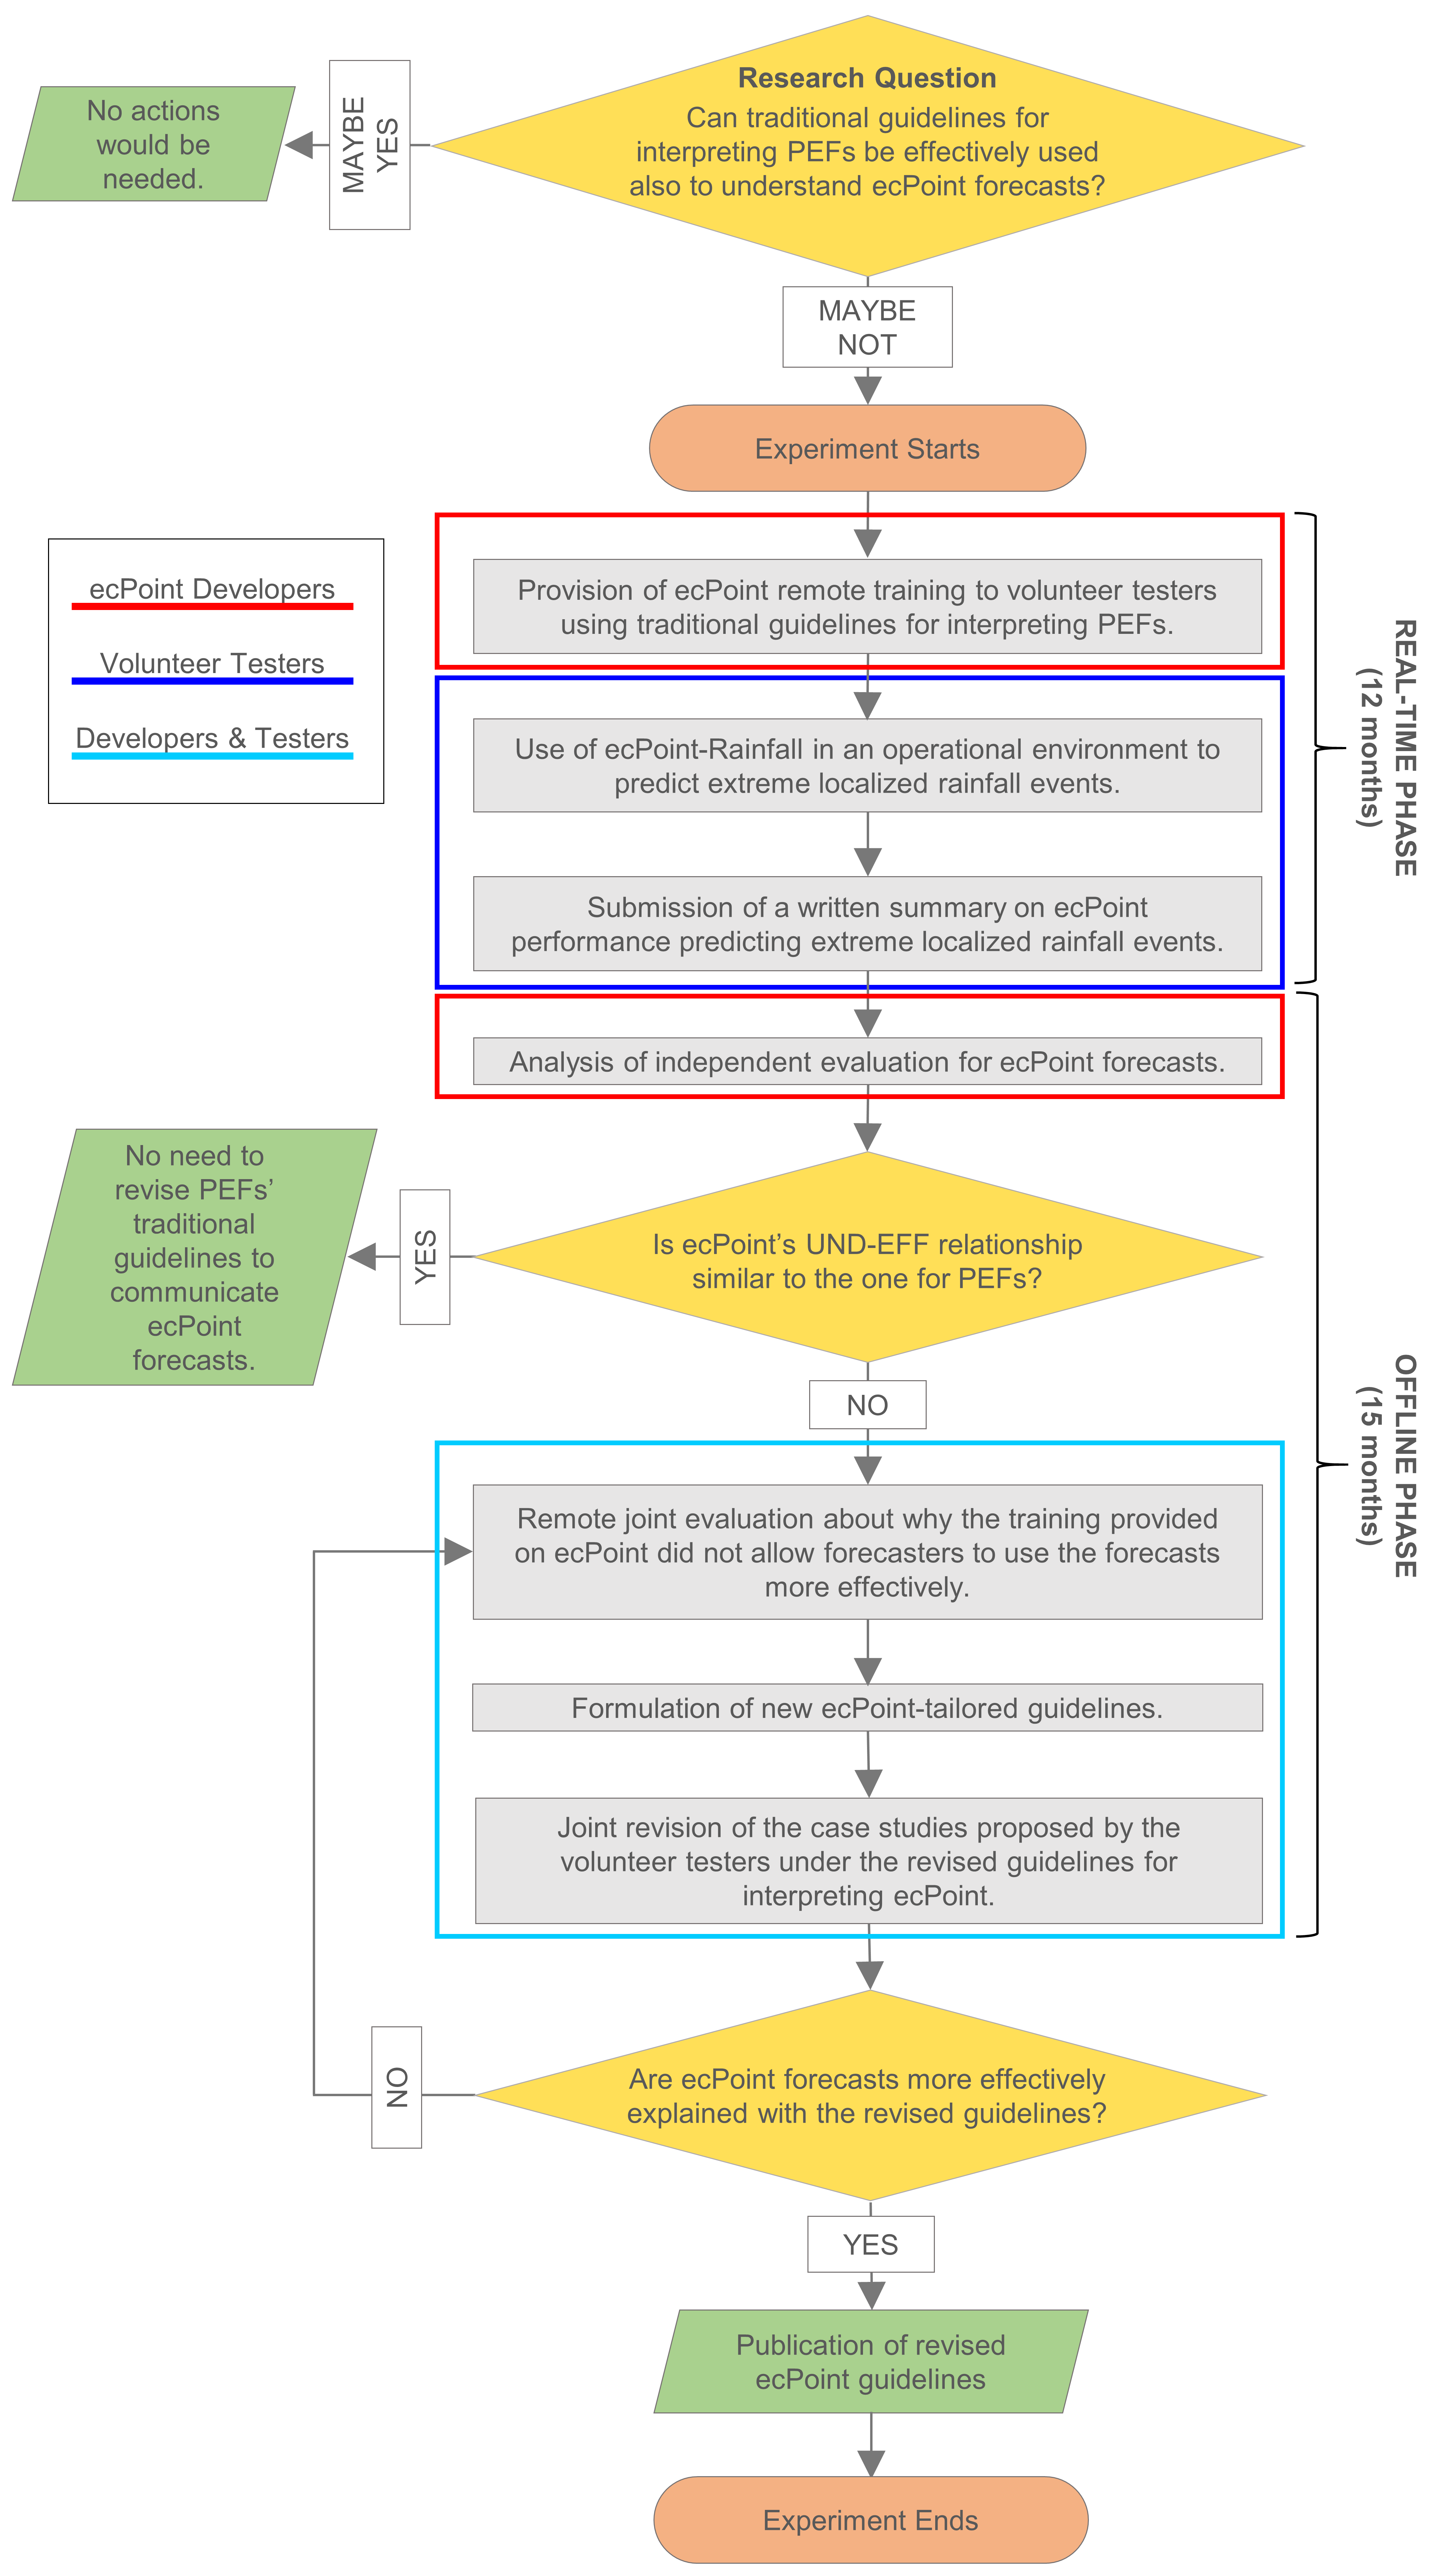
\includegraphics[width=19pc]{manuscript/Figures/FlowChart.png}}
\caption{Firstly, the flowchart describes the experiment processes that follow in the two experiment phases (real-time and offline). Secondly, the flowchart describes who, between developers (red squares), testers (blue squares) and developers & testers (cyan squares), conducted the experiment processes. Finally, the flowchart describes the possible experiment outcomes.}
\label{FlowChart}
\end{figure}

\begin{figure*}
\centerline{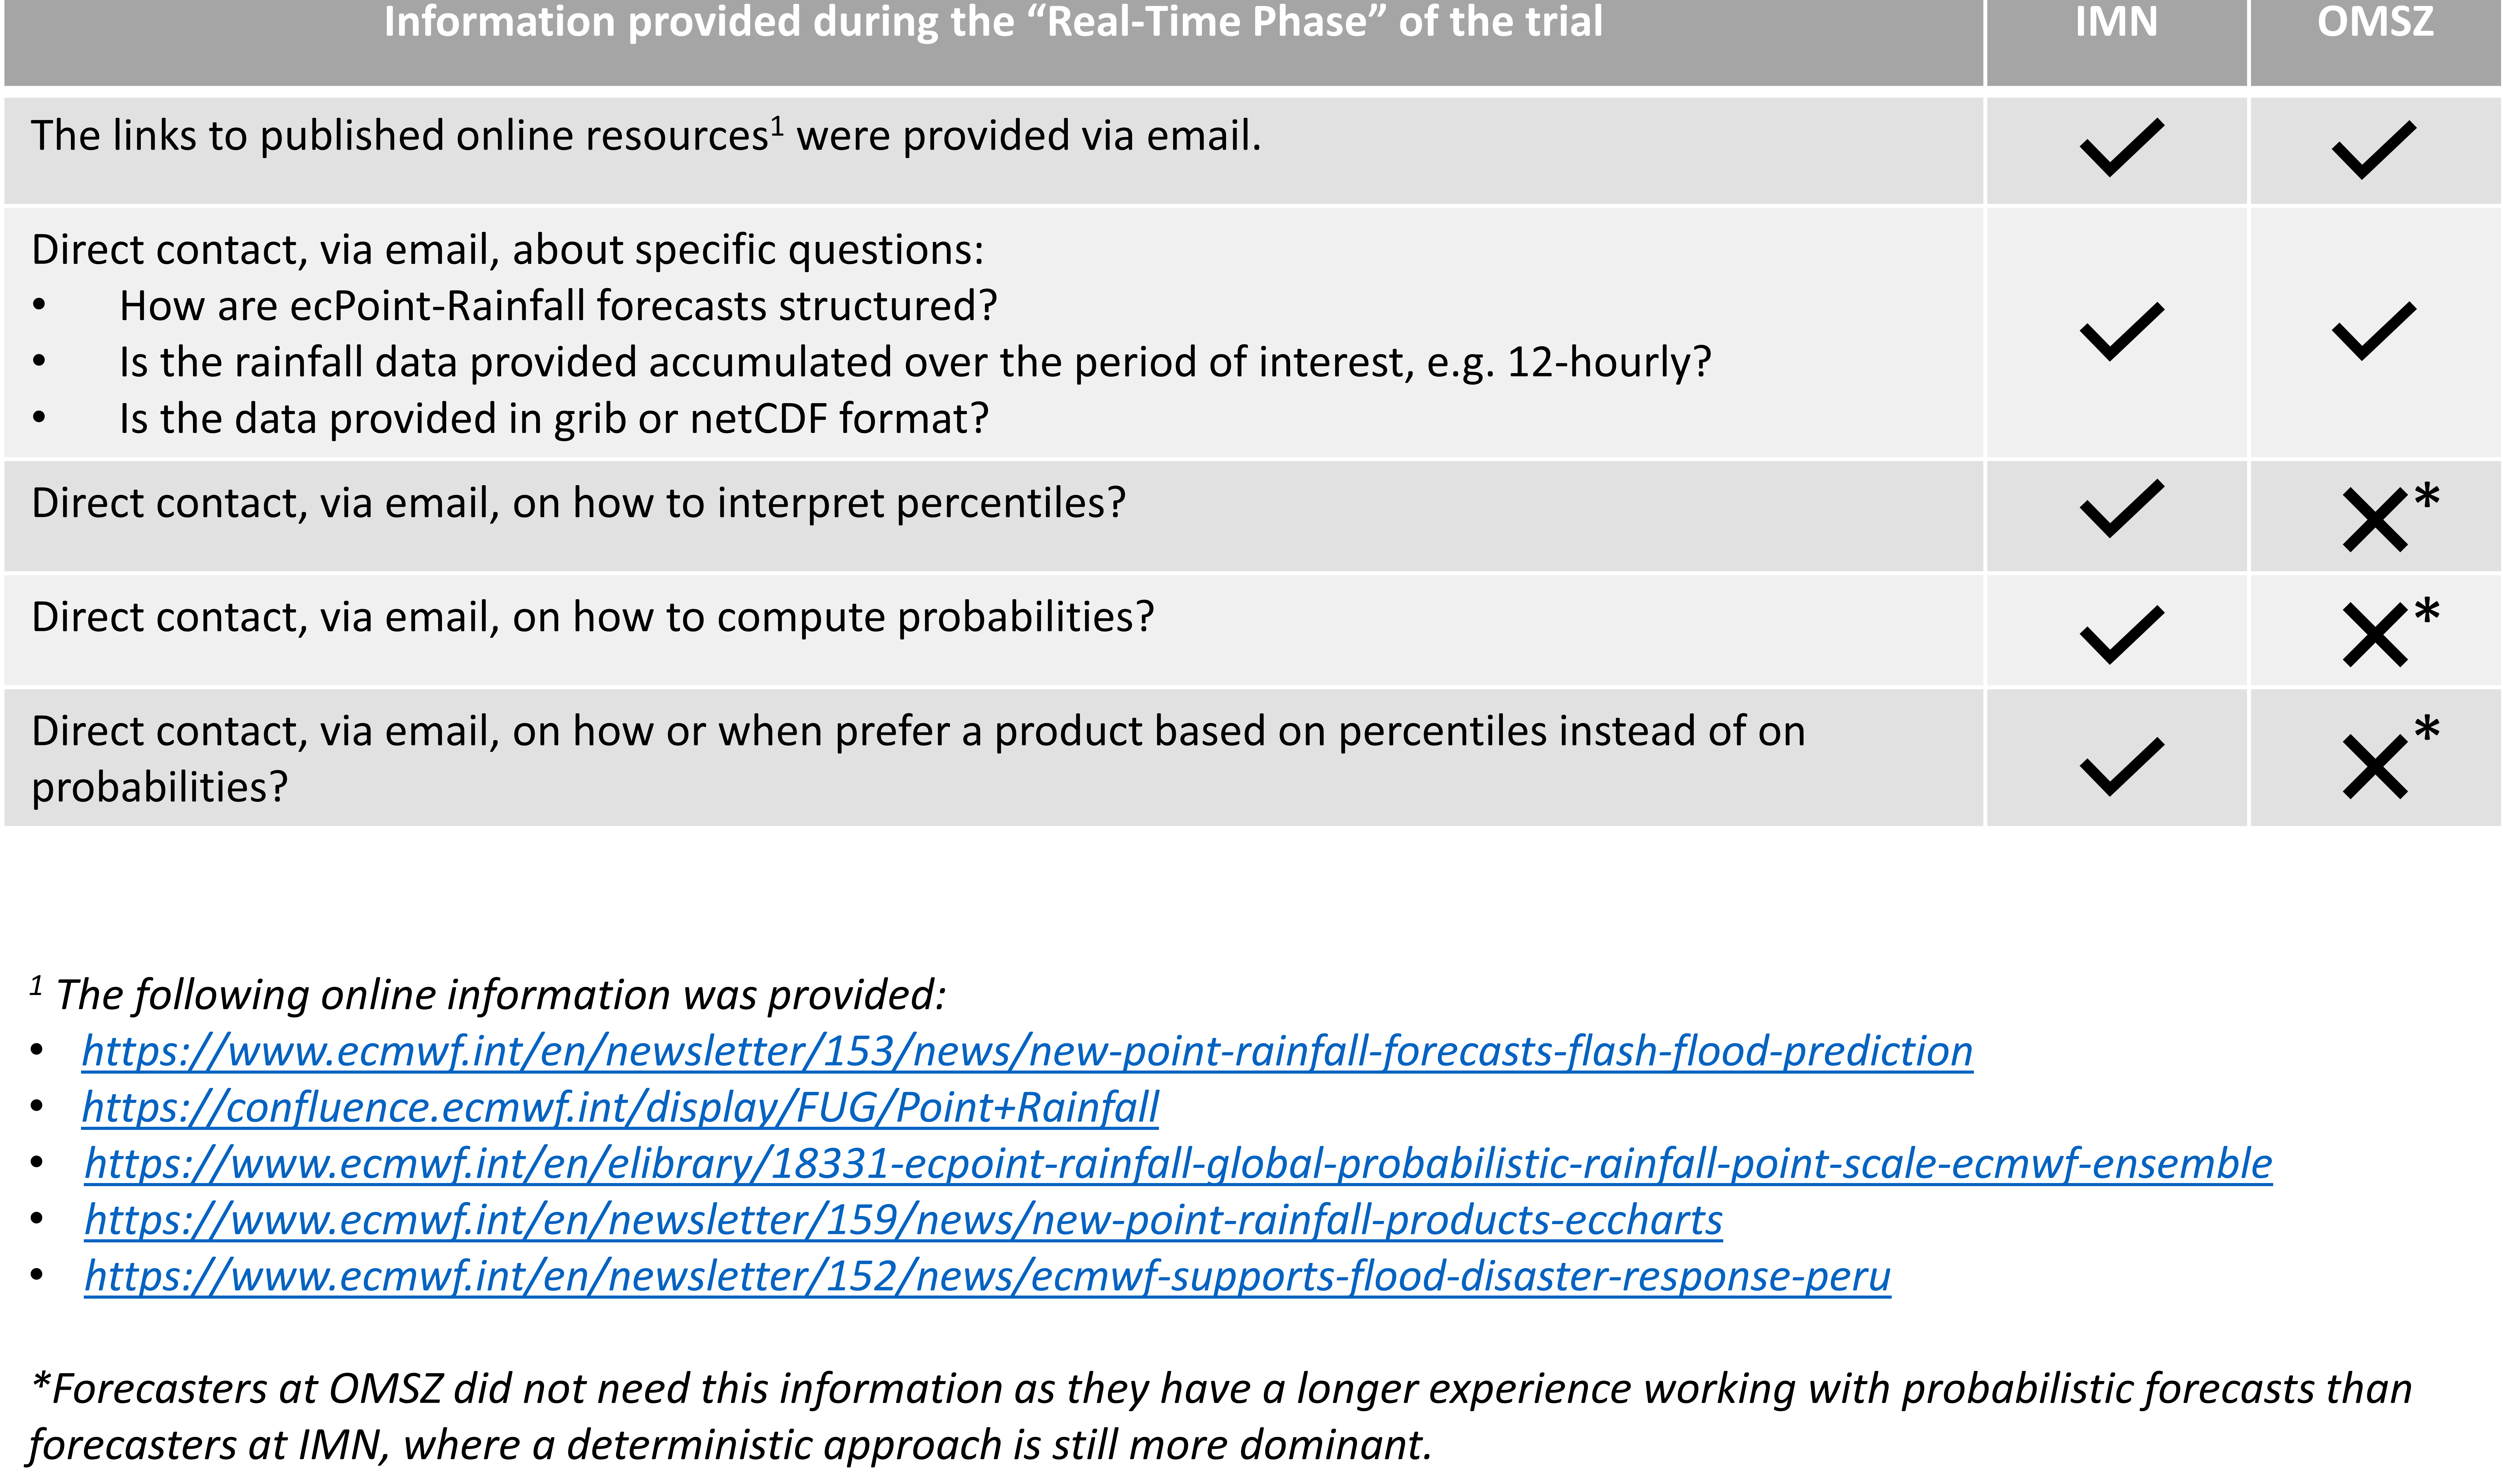
\includegraphics[width=39pc]{manuscript/Figures/Remote_Training.png}}
\caption{Training material provided to IMN and OMSZ at the beginning of the "Real-Time Phase" of the trial.}
\label{Fig5}
\end{figure*}
 

%%%%%%%%%%%%%%%%%%%%
% Results
\section{Results: real-time phase}

\subsection{Costa Rica}

\subsubsection{Products created for forecasters}
\begin{figure}
\centerline{\includegraphics[width=39pc]{manuscript/Figures/.jpg}}
\caption{Panel (a) shows the climate regions of Costa Rica defined by IMN. Panels from (o-1) to (o-6) show 12-hourly rainfall observations between October 3rd and 5th, 2018. Panels from (i-1) to (i-3) show the impacts caused by the extreme event in the regions in which CNE declared the state of red alert (the photos come from www.teletica.com).}
\label{Fig5}
\end{figure}





\subsubsection{Subjective Verification}

\begin{figure*}
\centerline{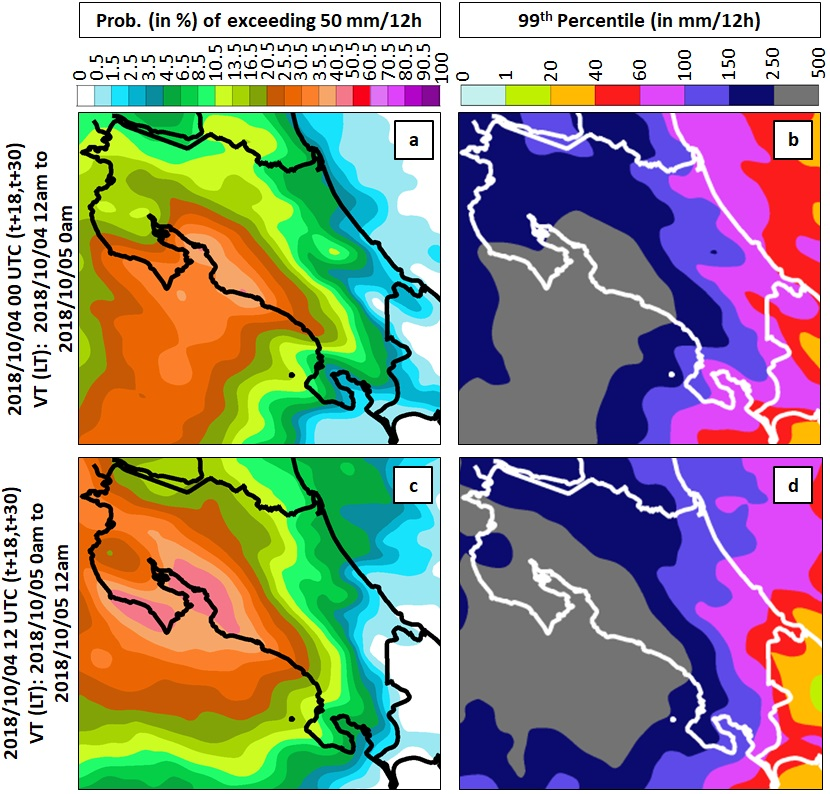
\includegraphics[width=39pc]{manuscript/Figures/Fig5.jpg}}
\caption{Panel (a) shows the climate regions of Costa Rica defined by IMN. Panels from (o-1) to (o-6) show 12-hourly rainfall observations between October 3rd and 5th, 2018. Panels from (i-1) to (i-3) show the impacts caused by the extreme event in the regions in which CNE declared the state of red alert (the photos come from www.teletica.com).}
\label{Fig5}
\end{figure*}


\begin{figure}
\centerline{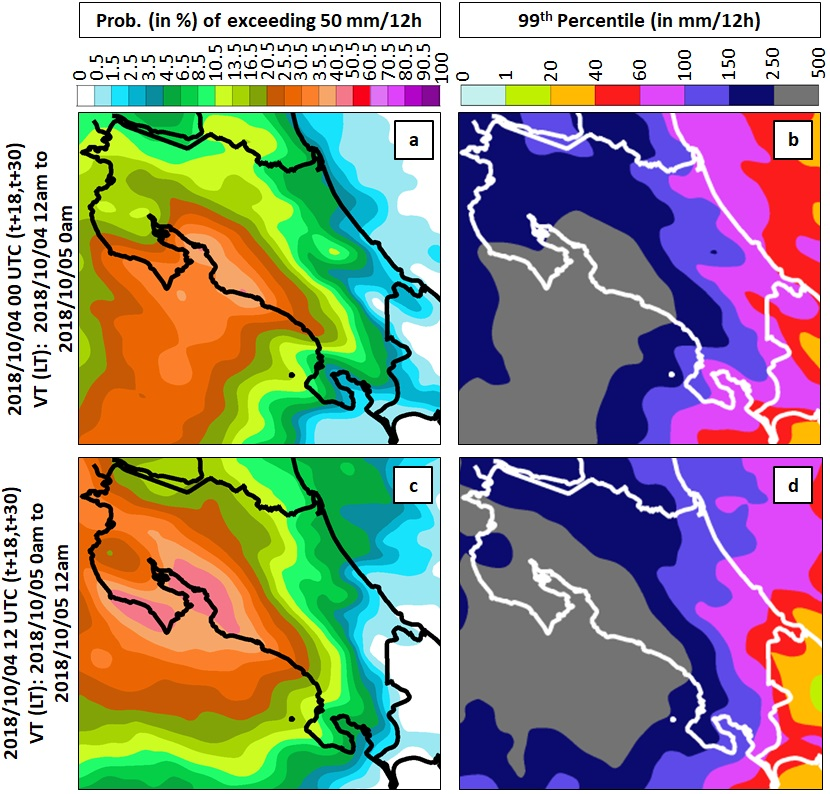
\includegraphics[width=19pc]{manuscript/Figures/Fig6.jpg}}
\caption{Panels (a) and (c) show the probabilities of not exceeding 50 mm/12h, and panels (b) and (d) show the 99th percentile, both for ecPoint-Rainfall forecasts. Panels (a) and (b) correspond to the forecast on 2018/10/04 at 00 UTC (t+18,t+30), which correspond to the period between 2018/10/04 12am and 201/10/05 0am (local time). Panels (c) and (d) correspond to the forecast on 2018/10/04 at 12 UTC (t+18,t+30), which correspond to the period between 2018/10/05 0am and 201/10/05 12am (local time).} 
\label{Fig6}
\end{figure}


\begin{figure*}
\centerline{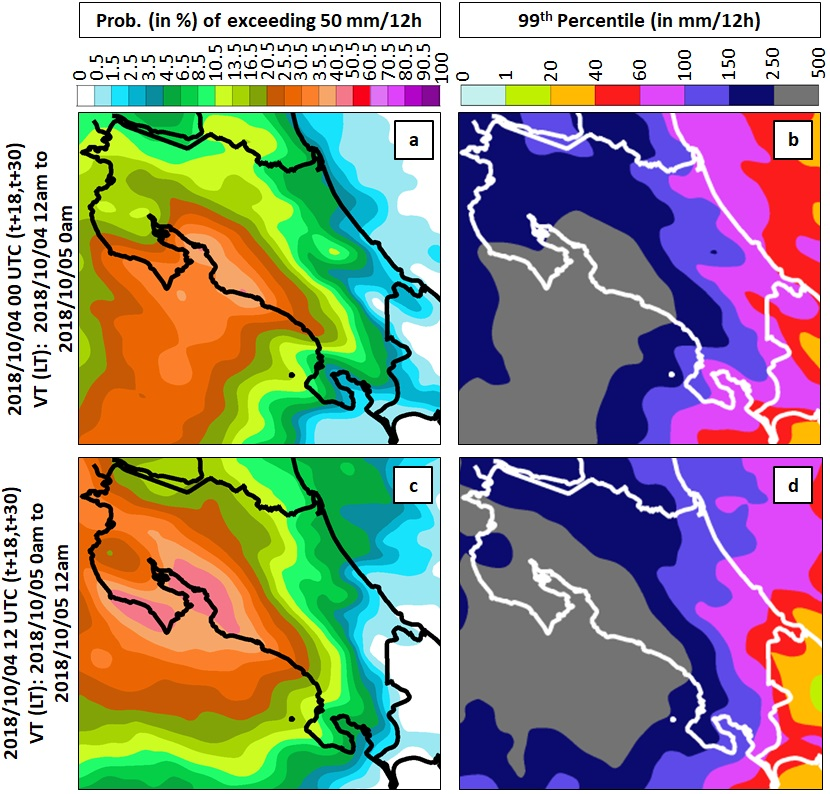
\includegraphics[width=39pc]{manuscript/Figures/Fig7.jpg}}
\caption{Forecast evolution (from day 7 to day 1) for the rainfall event occurred between October 04th at 12am and October 5th at 0am (see Fig. \ref{Fig4}o-4 to compare the forecasts with the observations). From the left, the first column shows the 85th percentile for ecPoint-Rainfall, the second column shows the 85th percentile for the raw ENS, the third column shows the 99th percentile for ecPoint-Rainfall, the fourth column shows the wettest member of the raw ENS, and the fifth column shows the deterministic forecast from WRF-1.5 provided by IMN (spatial resolution of 1.5 km). The shown raw ECMWF ENS and ecPoint-Rainfall forecasts correspond to runs at 12 UTC, which is the first available run from Europe to IMN forecasters due to time difference (UTC-6) between Europe and America. The displayed WRF-1.5 forecasts correspond to runs at 18 UTC, which is the first run available to IMN forecasters in the morning for their in-house models.}
\label{Fig7}
\end{figure*}


\begin{figure}
\centerline{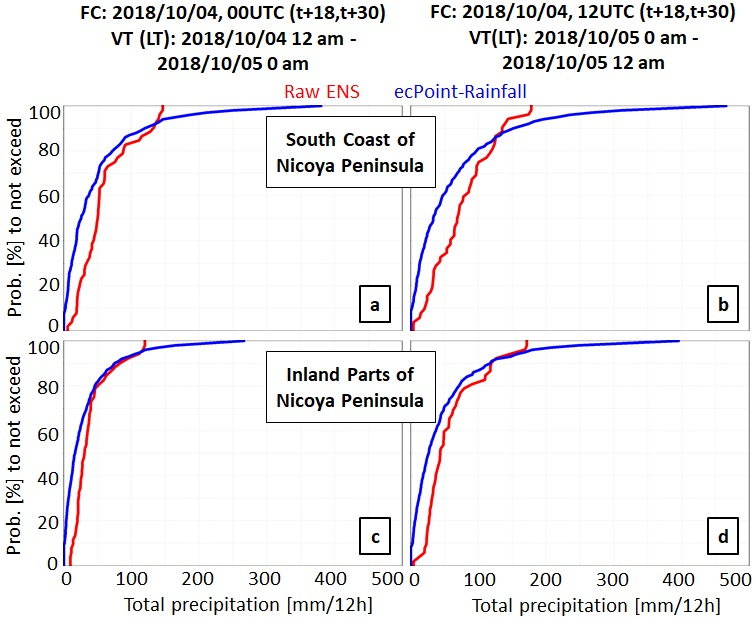
\includegraphics[width=19pc]{manuscript/Figures/Fig8.jpg}}
\caption{CDFs for ecPoint-Rainfall (in blue) and raw ENS (in red). Panels (a) and (b) display the CDFs for a location representative of the south coast of the Nicoya peninsula (lat=9.82,lon=-84.94). Panels (c) and (d) display the CDFs for a location representative of the inland parts of the Nicoya peninsula (lat=10.08,lon=-85.47). Panel (a) and (c) correspond to the forecast on 2018/10/04 at 00 UTC (t+18,t+30), which correspond to the period between 2018/10/04 12am and 201/10/05 0am (local time). Panel (b) and (d) correspond to the forecast on 2018/10/04 at 12 UTC (t+18,t+30), which correspond to the period between 2018/10/05 0am and 201/10/05 12am (local time).}
\label{Fig8}
\end{figure}

\subsection{Hungary}


\section{Results: offline phase}

\begin{figure*}
\centerline{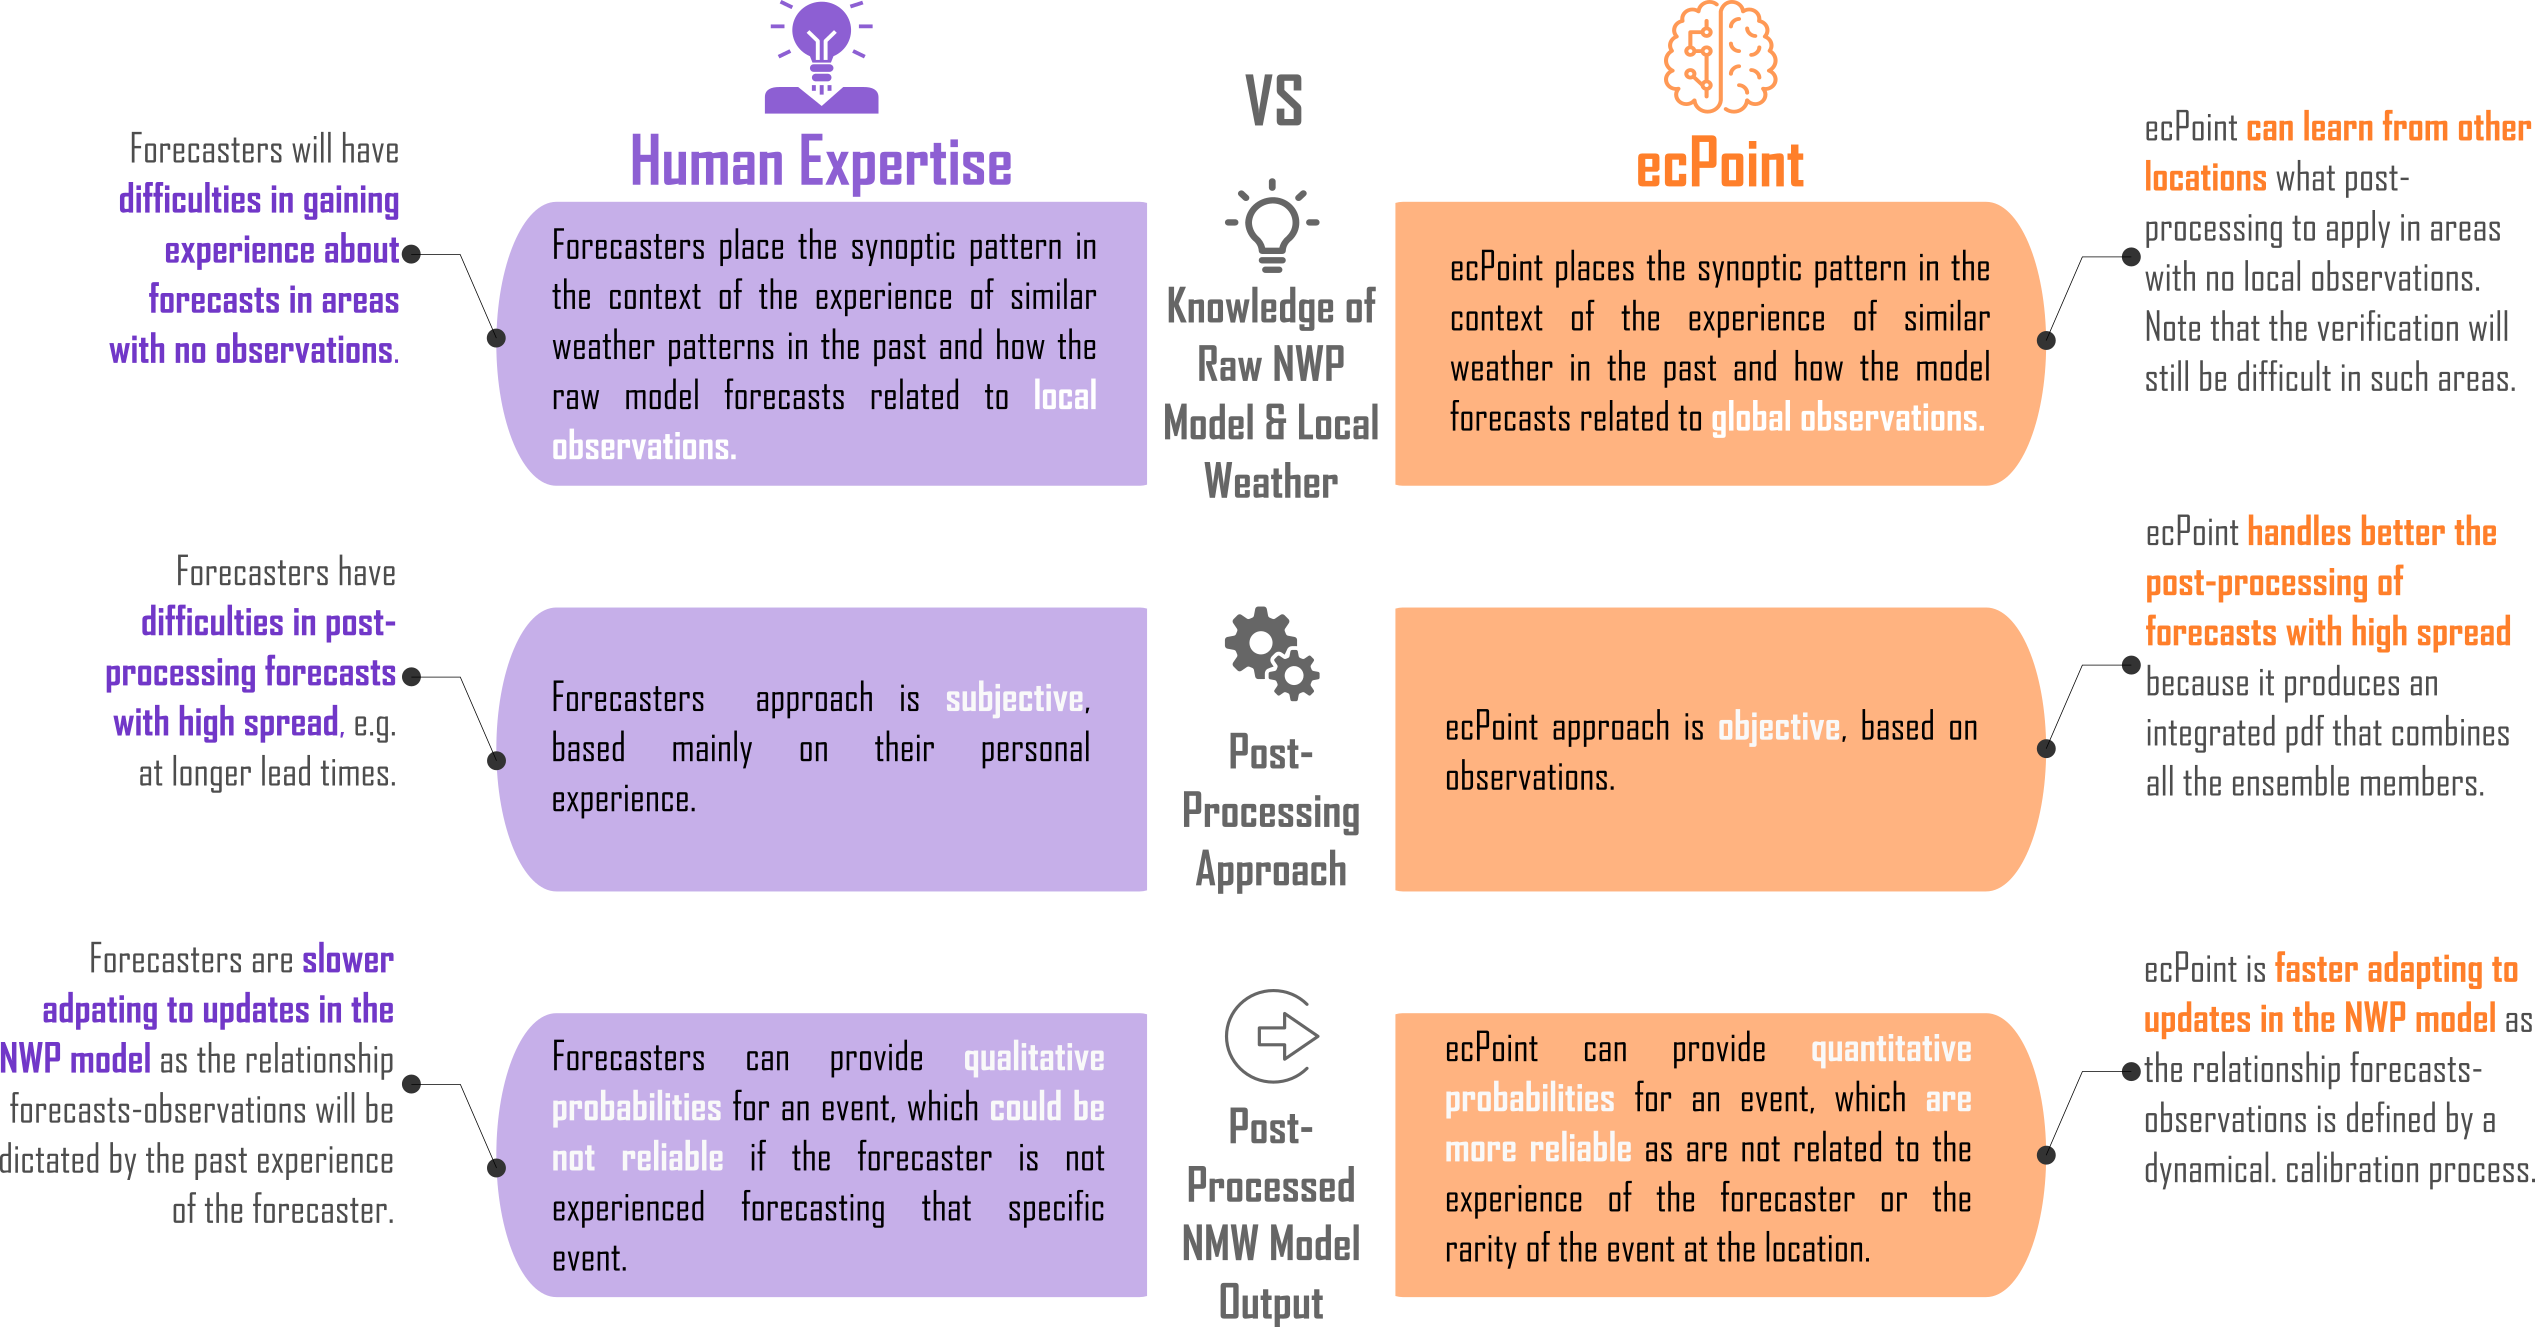
\includegraphics[width=39pc]{manuscript/Figures/Fig9.png}}
\caption{Comparison of approaches for forecasts adjustments: expert human adjustment vs. ecPoint.}
\label{Fig.9}
\end{figure*}






%%%%%%%%%%%%%%%%%%%%
% Discussions
\section{Discussion}


%%%%%%%%%%%%%%%%%%%%
% Conclusions
\section{Conclusion}


%%%%%%%%%%%%%%%%%%%
% ACKNOWLEDGMENTS %
%%%%%%%%%%%%%%%%%%%
\acknowledgments


%%%%%%%%%%%%%%%%%%%%%%%%%%%%%%%
% DATA AVAILABILITY STATEMENT %
%%%%%%%%%%%%%%%%%%%%%%%%%%%%%%%
\datastatement
The data that support the findings of this study are available from the corresponding author upon request.


%%%%%%%%%%%%%%
% REFERENCES %
%%%%%%%%%%%%%%
\bibliographystyle{ametsoc2014}
\bibliography{references}

\end{document}